

\section{下载与安装}

\subsection{下载 Python}
首先，请访问 Python 官方网站 \url{https://www.python.org/downloads/release/python-31210/}。

将页面滑倒最下面，找到适合你操作系统的安装包进行下载。通常 Windows 用户选择 "Windows installer (64-bit)"。

\begin{figure}[H]
    \centering
    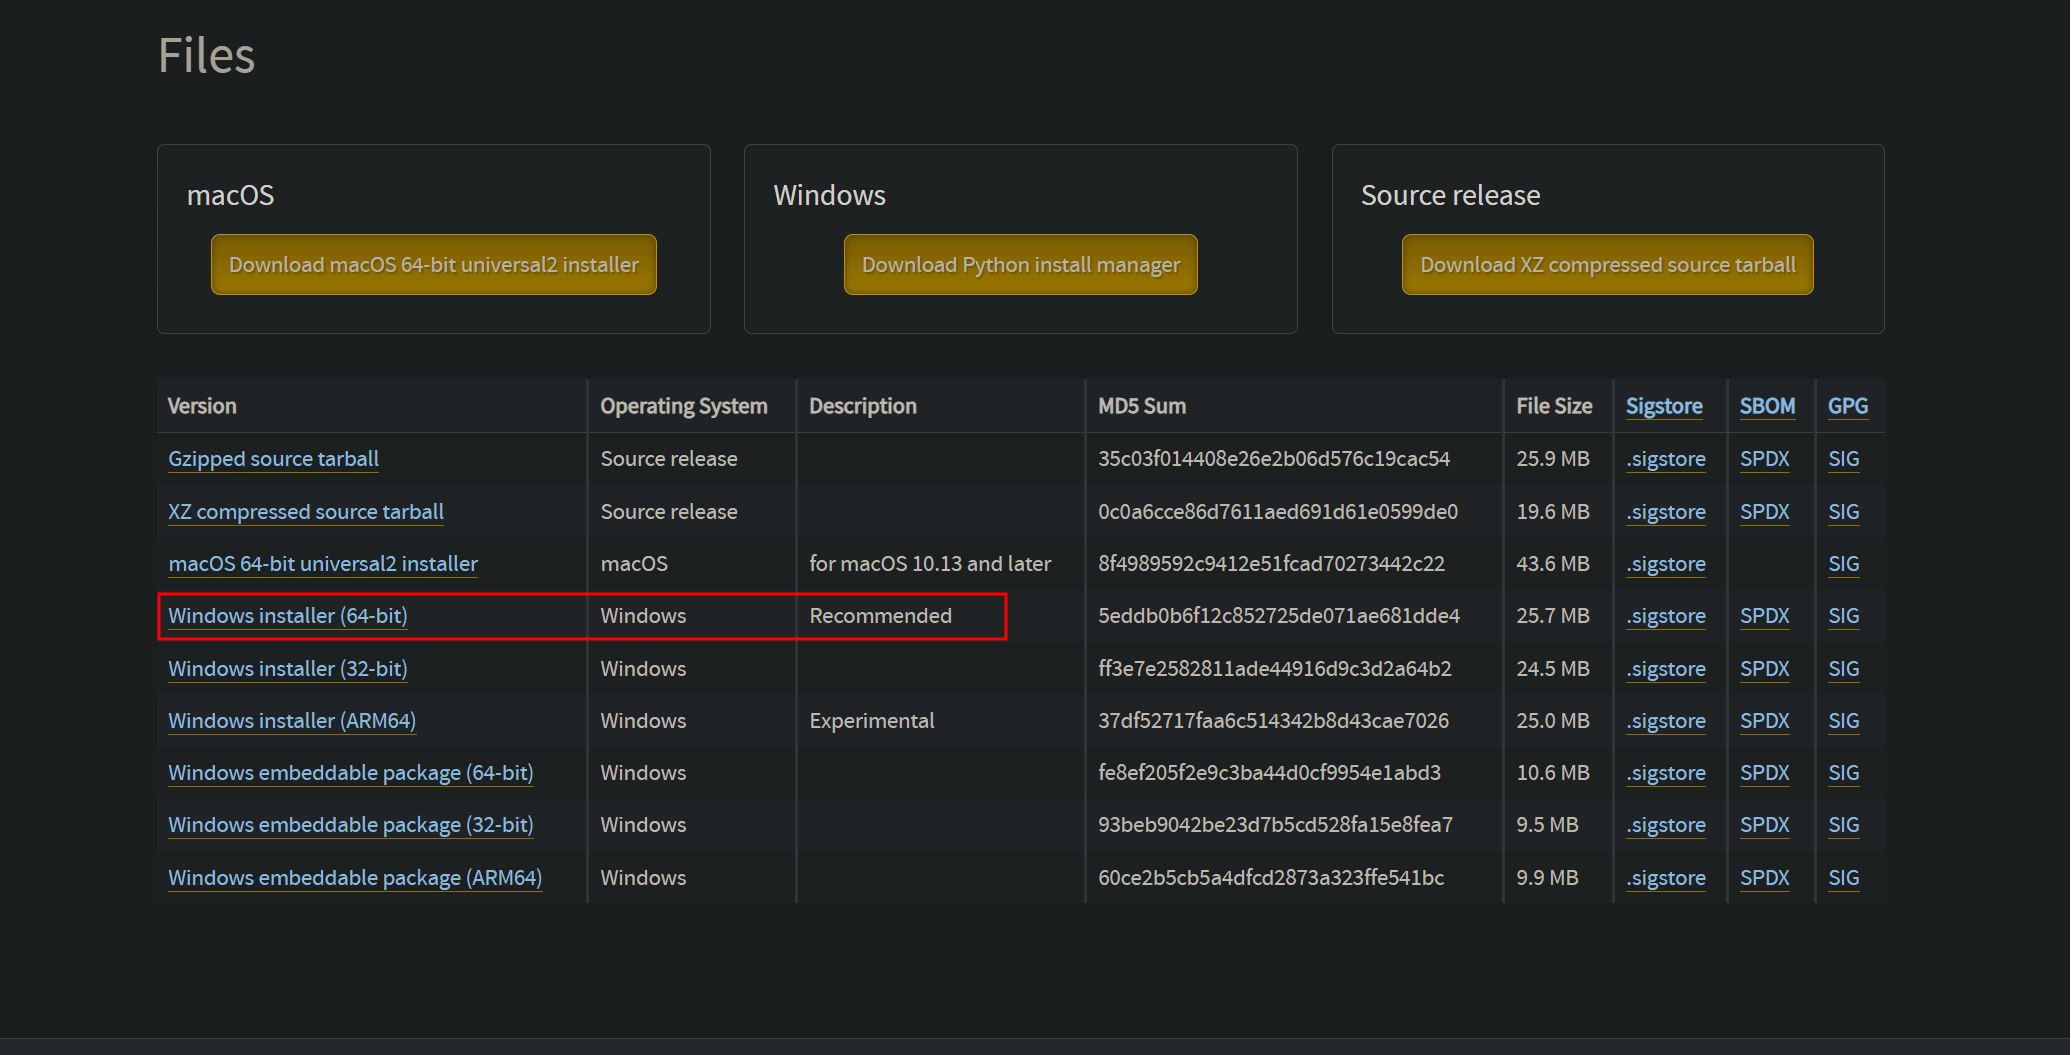
\includegraphics[width=0.8\linewidth]{figures/网站安装包位置.png}
    \caption{Python 官网下载位置}
    \label{fig:download_location}
\end{figure}
\newpage


\subsection{安装步骤}

\subsubsection{启动安装程序}




\begin{enumerate}[label=\ding{\numexpr171+\arabic*}]
 \item 双击下载的安装包，启动安装程序。
 


 \item \textbf{重要提示：} 在安装界面的底部，务必勾选 \textbf{Add Python to PATH} 选项。这将允许你在命令行中直接运行 Python。



 \item 然后，你可以选择 \textbf{Install Now} 进行默认安装，
 或者选择 \textbf{Customize installation} 进行自定义安装。


那么如果你有选择困难症，我推荐你选 \textbf{Customize installation}（自定义安装）。
理由如下：

\vspace{1em}
如果你追求长远管理、高自由度和稳定性，并且你有专门存放软件
的 D: 盘习惯（这非常好），那么一定要选下面
的【Customize installation】（自定义安装）。

这种方式可以让你避开系统盘深层的 AppData 目录，防止未
来 C 盘爆满，也方便你手动管理环境。也可以让你完全按照我的
教程来设置，避免一些莫名其妙的问题。


\begin{figure}[H]
    \centering
    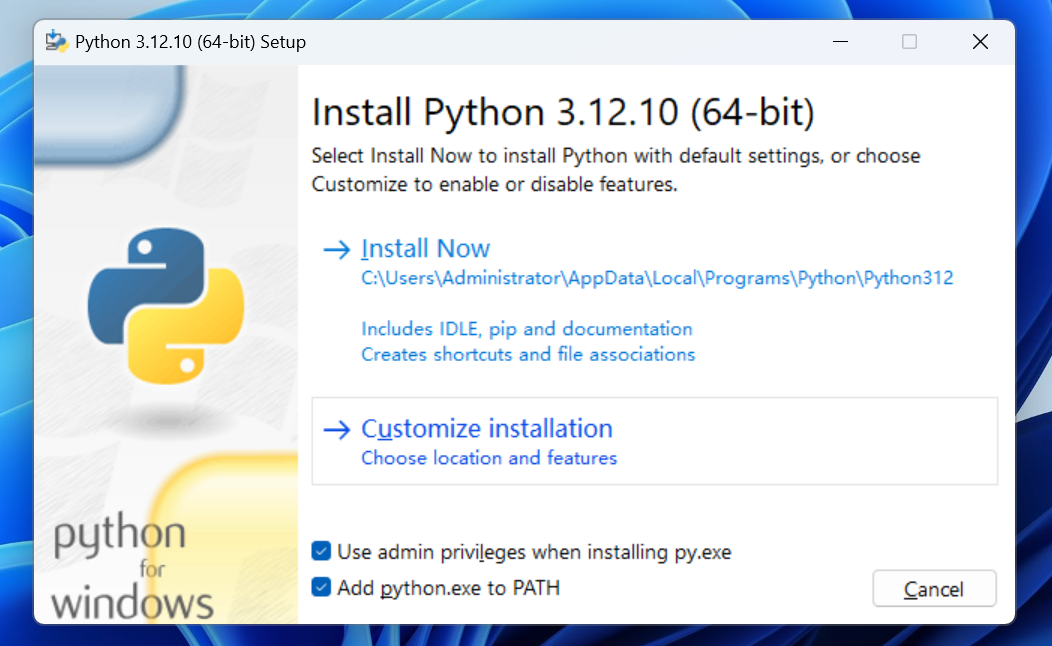
\includegraphics[width=0.8\linewidth]{figures/Python安装窗口1.png}
    \caption{启动安装程序，务必勾选 Add Python to PATH}
    \label{fig:install_step1}
\end{figure}

\end{enumerate}

\newpage



\subsubsection{选择可选功能}
在 Optional Features 界面，建议保持默认全选。特别是 \textbf{pip}（Python 包管理工具）和 \textbf{IDLE}（Python 自带的开发环境）是非常重要的组件。

\begin{figure}[H]
    \centering
    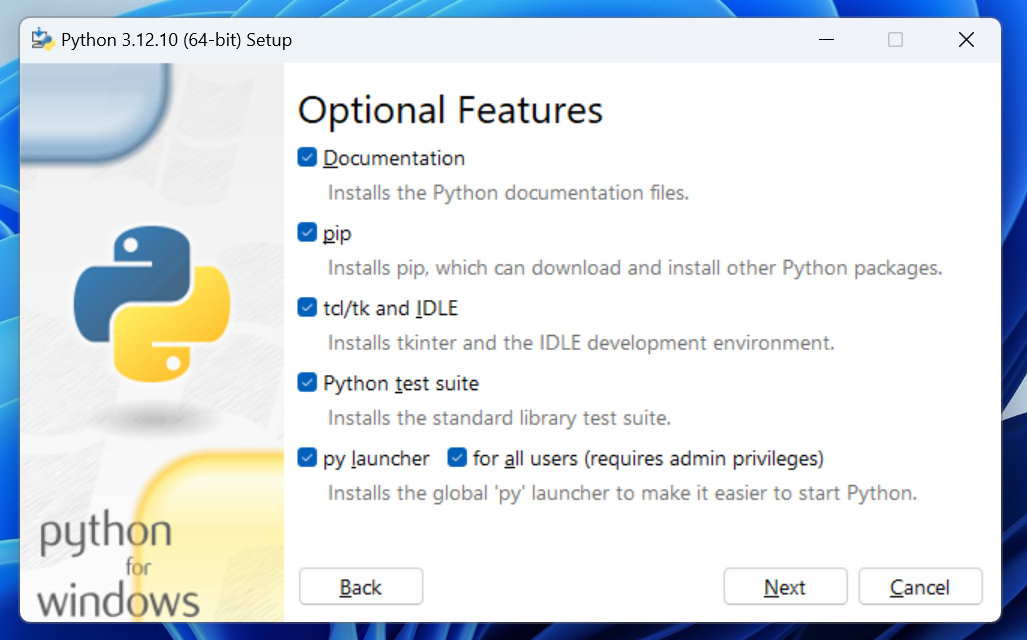
\includegraphics[width=0.8\linewidth]{figures/Python安装窗口2.png}
    \caption{选择可选功能}
    \label{fig:install_step2}
\end{figure}



\subsubsection{高级选项}选
在 Advanced Options 界面，你可以选择安装路径。如果你希望
所有用户都能使用 Python，可以勾选 \textbf{Install for all users}（
\textcolor{red}{建议勾选}）。

\paragraph{关于调试选项}
界面中还有 \textbf{Debugging symbols} (调试符号) 和 
\textbf{Debug binaries} (调试版二进制文件) 两个选项。\textcolor{red}{建议不勾选}
\begin{itemize}
    \item \textbf{这是什么？} 它们主要用于开发 Python 扩展模块（C/C++ 编写）或深入调试 Python 解释器本身崩溃问题。
    \item \textbf{有没有必要安装？} 对于绝大多数 Python 学习者和开发者来说，\textbf{完全不需要}。它们会占用大量磁盘空间，且日常写 Python 代码用不到。
    \item \textbf{谁一定需要？} 只有当你需要编写 C/C++ 扩展，或者你是 Python 核心开发者需要调试解释器源码时，才需要勾选。
\end{itemize}



\paragraph{路径设置建议}
为了方便以后管理（比如明年你想装个 Python 3.13 玩玩），建议优化安装路径结构。
（\textcolor{red}{建议自定义一个安装路径}）


那么当你开始自定义安装路径时，你可能会犯一个毛病。
你可能会习惯性地把 Python 装在类似下面的路径：
现在的路径可能是：\texttt{D:\textbackslash Personal\_Software\textbackslash Python} (这样安装会让 python.exe 直接散落在 Python 文件夹里，以后如果有其他版本就乱了)。

建议修改为： 👉 \texttt{D:\textbackslash Personal\_Software\textbackslash Python\textbackslash Python312} (手动在后面打字加上 \textbackslash Python312)。

这样，Python 3.12 就会乖乖待在它专属的文件夹里，既整洁又专业。
推荐的目录结构如下：

\begin{verbatim}
Personal_Software/
    └── Python/
        ├── Python312/   <-- 本次安装位置
        ├── Python313/   (未来可能安装的版本)
        └── Python314/   (不同版本互不干扰)
\end{verbatim}

确认设置无误后，点击 \textbf{Install} 开始安装。

\begin{figure}[H]
    \centering
    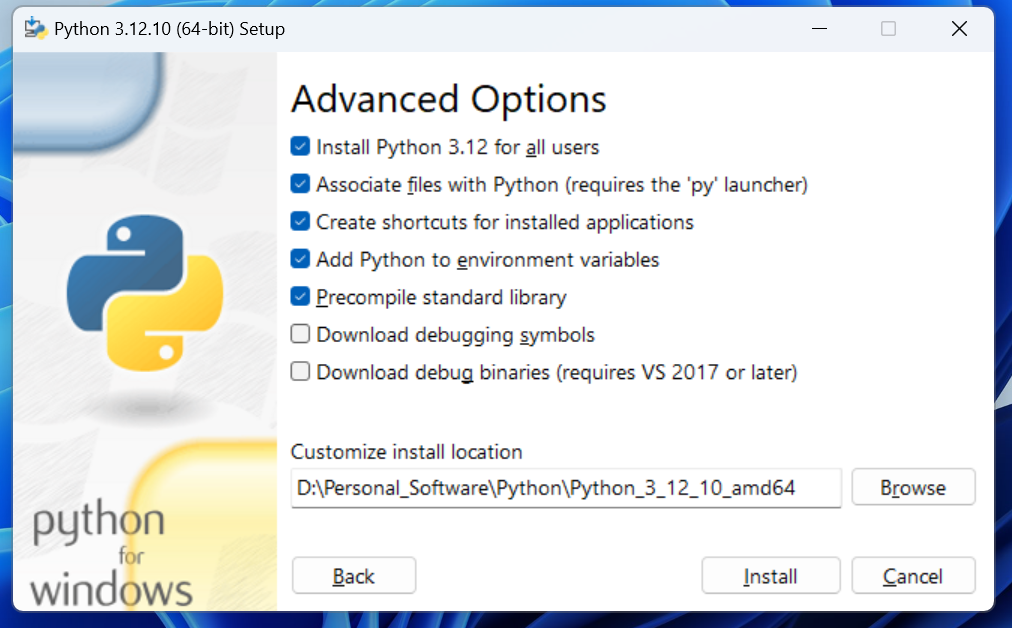
\includegraphics[width=0.8\linewidth]{figures/Python安装窗口3.png}
    \caption{高级选项设置}
    \label{fig:install_step3}
\end{figure}


\newpage

\subsubsection{等待安装完成}
安装程序将自动复制文件并配置环境，请耐心等待进度条完成。

\begin{figure}[H]
    \centering
    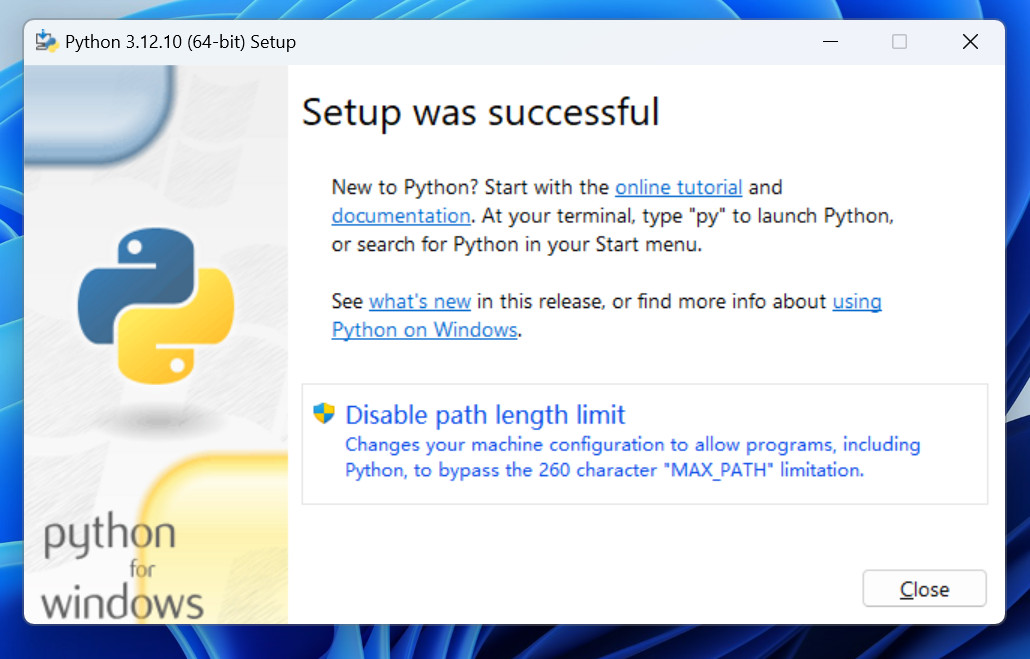
\includegraphics[width=0.8\linewidth]{figures/Python安装窗口4.png}
    \caption{正在安装}
    \label{fig:install_step4}
\end{figure}


当看到 "Setup was successful" 的提示时，表示安装已完成。

如果界面上出现 \textbf{Disable path length limit} 的选项，建议点击它。这将解除 Windows 对文件路径长度的限制，避免某些深层目录下的文件无法访问的问题。

最后点击 \textbf{Close} 关闭安装程序。

\begin{figure}[H]
    \centering
    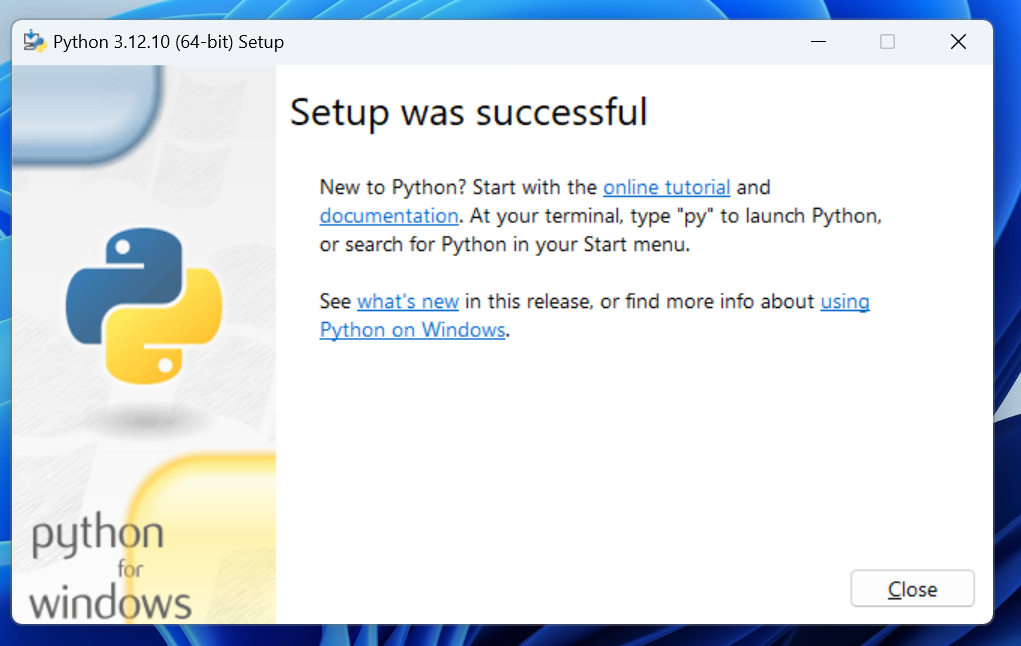
\includegraphics[width=0.8\linewidth]{figures/Python安装窗口5.png}
    \caption{安装成功}
    \label{fig:install_step5}
\end{figure}
\newpage